\subsection{Drell-Yan}

The Drell-Yan process was proposed in 1970 to describe the
cross-section where the final state results in two oppositely charged
leptons \cite{DY_process}.  The process involves the annihilation of a
quark and an anti-quark into a virtual photon, Z-boson or W-boson
which then decays into a lepton and an anti-lepton pair.  The 2015
COMPASS specific Drell-Yan reaction is given in
equation~\ref{equ:ComDY} and the correspond Feynman diagram is given in figure~\ref{fig:fey_DY}.
%
\begin{equation}
  H_a(P_a) + H_b(P_b, S_b) \rightarrow \gamma ^*(q) + X \rightarrow l^-(l) + l^+(l') + X
  \label{equ:ComDY}
\end{equation}
%
Here $H_{a(b)}(P_{a(b)}, S_b)$ represents the initial state hadron as
a function of momentum and spin, $\gamma^{*}$ is a virtual photon,
$l^{+(-)}$ are the measured final state leptons and $X$ represents
what is not measured.  In all cases subscript a(b) will refer to the
beam(target).  Specifically the leptons studied at COMPASS were final
state muons because the long range of muons makes muons easier to study experimentally. Kinematic variables of
interest in the Drell-Yan process are as shown in
equations~\ref{equ:s}-~\ref{equ:M2}.

\begin{subequations}
  \begin{align}
    &s = (P_a + P_b)^2    & \text{Center of momentum energy squared.}\label{equ:s}\\
    &x_{a(b)} = \frac{q^2}{P_{a(b)} \cdot q} & \text{x-Bjorken, parton longitudinal momentum fraction.} \\
    &x_f = x_a - x_b & \text{x-Feynman variable.}\\
    &M^2 = q^2 = sx_ax_b & \text{Invariant mass of the virtual photon.}\label{equ:M2}
  \end{align}
  \label{equ:DYkin}
\end{subequations}

\begin{figure}
  \includegraphics[width=0.5\textwidth,center]{feyDY}
  \caption{}{The Drell-Yan Feynman diagram for (un)polarized
    (beam)target where $\bar{u}$ and $u$ are the annihilating quarks
    and the invariant mass is low enough so only an electro-magnetic
    reaction can occur.}
  \label{fig:fey_DY}
\end{figure}

One of the defining characteristics of the Drell-Yan process is a
steep falloff of the cross-section as function of the invariant mass
of the process.  Above 4 $\frac{GeV}{c^2}$ the cross-section is on the
order of nano-barns making the Drell-Yan process experimentally
challenging.  This implies the beam intensity required to study this
process must be quit high and at the same time the background must be
well suppressed.  From the theoretical point of view, however, the
Drell-Yan process is considered to be cleaner than other processes
including SIDIS.  This is due to the fact that only initial state
soft, non-perturbative terms describe the process.  There are no final
state quarks leading to the need for non-perturbative fragmentation
functions.  The only soft terms come from the parton distribution
functions (PDF) of the incoming hadrons. \par

One of the most interesting features of the Drell-Yan process is its
ability to describe transverse momentum dependent distributions.
Through the Drell-Yan process with the transversely polarized target
and an unpolarized beam, as in the 2015 COMPASS data taking, there is
the possibility to extract the Sivers function, the Boer-Mulders
function, the Prezelosity function and the Transversity function.  The
leading order Drell-Yan cross-section for an unpolarized beam on a
transversely polarized target is given in equation~\ref{DY-xsection}
\cite{proposal}.

\begin{dmath}
\frac{d\sigma}{d^4qd\Omega} = \frac{\alpha^2_{em}}{Fq^2}\hat{\sigma}_U
\Bigg \{ \Big(1 + D_{[\sin^2(\theta)]}A_U^{\cos(2\phi)}\cos(2\phi)\Big )
+ \| S_T \| \Big [ A_T^{\sin(\phi_S)}\sin(\phi_S) +
  D_{[\sin^2(\theta)]}\Big
  (A_T^{\sin(2\phi+\phi_S)}\sin(2\phi+\phi_S)+A_T^{\sin(2\phi-\phi_S)}\sin(2\phi-\phi_S)\Big
  ) \Big ] \Bigg \}
\label{DY-xsection}%
\end{dmath}
%
Where $F$ is the flux, $D_{[f(\theta)]}$ is a depolarization factor,
$\| S_t \|$ is transverse spin percentage and $\hat{\sigma}_U$ is the
unpolarized Drell-Yan cross-section.\par

To describe the different angles used in the Drell-Yan cross-section,
the description of the transversely polarized Drell-Yan process is
done in a target frame and a center of momentum frame called the
Collin-Sopers frame.  The target coordinate system,
figure~\ref{fig:TargFrame} is the frame where the beam is along the
z-axis and the virtual photon is along the x-axis.  The $\phi_S$ angle
know as phi Sivers is defined in the target frame.  The Collin-Sopers
coordinate system, figure~\ref{fig:CSframe} comes from boosting out of
the target frame along the z-axis and then boosting along the x-axis.
The Collin-Sopers frame gives the additional $\phi$ and $\theta$
angles used in the description of the cross-section
\cite{CollinSoperFrame}.

\begin{figure}
  \centering
  \begin{subfigure}[b]{0.47\textwidth}
    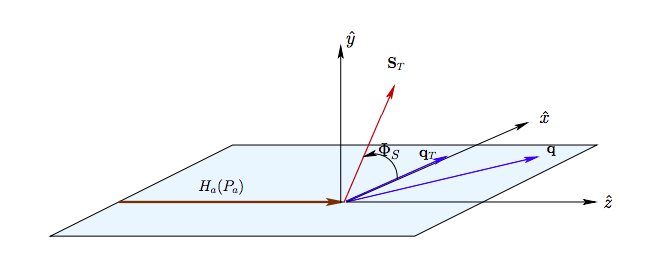
\includegraphics[width=\textwidth]{TargFrame}
    \caption{The target frame has the z-coordinate aligned with the
      incoming beam and the x-coordinate aligned with the virtual
      photon.}
    \label{fig:TargFrame}%
  \end{subfigure}
  \begin{subfigure}[b]{0.47\textwidth}
    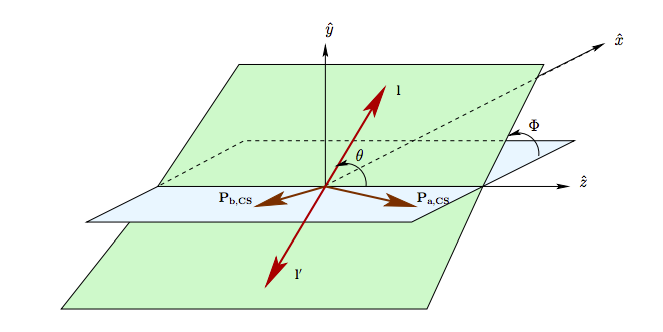
\includegraphics[width=\textwidth]{CSframe}
    \caption{The Collins-Soper frame is a center of momentum frame
      which can be reached from the target frame by a boost along the
      z-direction followed by boost in the x-direction.}
    \label{fig:CSframe}%
  \end{subfigure}
\end{figure}

Under the factorization theorem when the virtual photon invariant mass, $q^2$, is much greater than its transverse momentum, $q_T$, the cross-section amplitudes give a convolution of PDFs or TMDs of the beam and the target.  An example of this relation for the Sivers function is shown in equations~\ref{equ:Corr}-~\ref{equ:AT}.
%
\begin{subequations}
  \begin{align}
    \begin{split}
      C[w(k_{aT},k_{bT})f_a\bar{f}_b)] = \frac{1}{N_c}\sum_q e_q^2\int
      d^2k_{aT}d^2k_{bT}\delta^{(2)}(q_T - k_{aT}-k_{bT})w(k_{aT},
      k_{bT})\times\\ \Big [ f^q_a(x_a, k^2_{aT})f^{\bar q}_2(x_b,
        k^2_{bT}) + f^{\bar q}_1(x_a, k^2_{aT})f^q_2(x_b, k^2_{bT})
        \Big ] \quad \text{Correlation function.}\label{equ:Corr}
      \end{split}\\
    & F^1_U = C[f_a\bar{f}_b] \Repeat{11}{\qquad} \text{$F^1_U$ definition. }\\
    & A_T^{\sin(\phi_S)} = \frac{C[h \cdot k_{bT}f_a \bar{f}^{\perp}_{1T}]}{M_b F^1_U} \Repeat{5}{\qquad} \text{Sivers amplitude correlation.}\label{equ:AT}
  \end{align}
  \label{equ:SivCorr}
\end{subequations}
%
This means the Sivers function for the proton, $\bar{f}^{\perp}_{1T}$,
can be extracted from $A_T^{\sin(\phi_S)}$.  In a similar manor the
Prezelosity function comes from $A_T^{\sin(2\phi+\phi_S)}$, the
Transversity function from $A_T^{\sin(2\phi-\phi_S)}$ and Boer-Mulders
function from $A_U^{\cos(2\phi)}$.  Therefore from the cross-section
the Sivers, Prezelosity and Transversity functions can be extracted
from single spin asymmetries while the Boer-Mulders function can be
extracted from unpolarized Drell-Yan data. \par

